\chapter{التكاثر الجنسي عند النباتات الزهرية}\label{ch:b2:angiosperm-reproduction}

بستان تفاح في أيار أبيض بالزهر عالٍ بأزيز النحل؛ وفي تشرين الأول
تنوء الأشجار نفسها بالثمر، في كل تفاحة عشر بذور، وكل \omterm{def:b2:angiosperm-reproduction:seed}{بذرة} شجرة
جنينية ملفوفة في مخزون غذاء. وذلك التحول كله --- \omterm{def:b2:angiosperm-reproduction:flower}{الزهرة}، \omterm{def:b2:plant-life-cycles:heterospory}{واللقاح}
الذي تحمله حشرة، والأنبوب النامي عبر القلم، \omterm{prop:b2:angiosperm-reproduction:double}{والإلقاح المضاعف} الذي
يصنع في آن جنينًا ومؤونته، والمبيض المنتفخ ثمرةً مبنية لتُؤكل --- هو
الابتكار الذي جعل النباتات الزهرية، في مئة مليون سنة، نباتاتِ
اليابسة السائدة. يتناول هذا الفصل ذلك من \omterm{def:b2:angiosperm-reproduction:flower}{الزهرة} إلى \omterm{def:b2:angiosperm-reproduction:seed}{البذرة}
المنثورة.

\section{الزهرة}

\begin{definition}[أجزاء الزهرة]\label{def:b2:angiosperm-reproduction:flower}
\index{زهرة}\index{سداة}\index{كربلة}\index{مبيض}\index{ميسم}
\emph{الزهرة} ساق قصيرة تحولت أوراقها إلى أربع دوّارات. ففي الخارج
تحمي \emph{السبلات} (وهي معًا الكأس) البرعم؛ ثم \emph{البتلات}
(التويج)، وهي التي تُعلن؛ ثم \emph{السدى}، وكل سداة خيط يحمل
\emph{متكًا} فيه أربعة أكياس \omterm{def:b2:plant-life-cycles:heterospory}{لقاح}؛ وفي المركز \emph{كربلة} أو أكثر،
كل منها مطوية مختومة في \emph{مدقة} ذات \emph{ميسم} مستقبِل،
و\emph{قلم}، و\emph{مبيض} يحيط \emph{بالبييضات}. والزهرة التي فيها
سدى وكرابل \emph{خنثى} (وهو حال معظم الأنواع)؛ والنباتات
\emph{وحيدة المسكن} تحمل أزهارًا ذكرية وأنثوية منفصلة على فرد واحد
(الذرة، والبلوط، والبندق)، و\emph{ثنائية المسكن} تحملها على أفراد
منفصلة (البهشية، والصفصاف، ونخيل التمر). وكل مغزى الكربلة المغلقة
--- وهي الصفة التي سمّت كاسيات البذور --- أن البييضات محاطة: \omterm{def:b2:plant-life-cycles:heterospory}{فاللقاح}
لا يبلغها مباشرة أبدًا، بل عليه أن ينمو إليها عبر نسيج النبات، وهذا
يتيح للنبات أن يختار.
\end{definition}

\begin{omfigure}
\begin{tikzpicture}[every node/.style={font=\scriptsize}]
  % receptacle and pedicel
  \draw[thick] (0,-2.6) -- (0,-1.6);
  \draw[thick, fill=omExo!20] (-0.9,-1.6) .. controls (-1.0,-1.0) and (1.0,-1.0) .. (0.9,-1.6) -- cycle;
  % sepals
  \foreach \s in {-1,1} \draw[thick, fill=omExo!45] (0.6*\s,-1.4) .. controls (2.0*\s,-1.2) and (2.6*\s,-0.2) .. (2.8*\s,0.6) .. controls (2.0*\s,0.2) and (1.2*\s,-0.6) .. (0.6*\s,-1.4);
  % petals
  \foreach \s in {-1,1} \draw[thick, fill=omThm!15] (0.5*\s,-1.2) .. controls (1.6*\s,0.4) and (2.2*\s,1.8) .. (1.6*\s,3.0) .. controls (1.0*\s,2.0) and (0.5*\s,0.8) .. (0.5*\s,-1.2);
  % ovary with ovules
  \draw[thick, fill=omDef!12] (0,-0.7) ellipse (0.55 and 0.75);
  \foreach \p in {(-0.22,-0.5),(-0.22,-0.9),(0.22,-0.5),(0.22,-0.9)} \draw[thick, omDef, fill=omDef!40] \p circle (0.11);
  % style and stigma
  \draw[thick, fill=omDef!12] (-0.1,0.05) rectangle (0.1,1.9);
  \draw[thick, fill=omDef!40] (0,2.0) ellipse (0.28 and 0.14);
  % stamens
  \foreach \s in {-1,1} { \draw[thick] (0.35*\s,-1.0) .. controls (0.6*\s,0.2) .. (0.9*\s,1.5); \draw[thick, fill=omProp!60] (0.9*\s,1.6) ellipse (0.14 and 0.32); }
  % labels: right side
  \draw (0.28,2.0) -- (3.2,2.6) node[right] {ميسم};
  \draw (0.1,1.2) -- (3.2,1.9) node[right] {قلم};
  \draw (0.55,-0.6) -- (3.2,1.2) node[right] {مبيض};
  \draw (0.22,-0.9) -- (3.2,0.5) node[right] {بييضة};
  \draw (2.6,0.35) -- (3.2,-0.4) node[right] {سبلة};
  % labels: left side
  \draw (-1.5,2.4) -- (-2.6,2.8) node[left] {بتلة};
  \draw (-0.95,1.9) -- (-2.6,1.9) node[left] {متك};
  \draw (-0.65,0.6) -- (-2.6,0.9) node[left] {خيط};
  \draw (0,-2.2) -- (-2.6,-2.2) node[left] {التخت والحامل};
  \node[anchor=west, align=left] at (5.4,0.5) {ميسم + قلم + مبيض\\$=$ الكربلة (المدقة)};
  \node[anchor=west, align=left] at (5.4,-0.8) {متك + خيط\\$=$ السداة};
\end{tikzpicture}

{\small \omterm{def:b2:angiosperm-reproduction:flower}{زهرة} في مقطع طولي: سبلات وبتلات وسدى (خيط ومتك)، وفي
المركز \omterm{def:b2:angiosperm-reproduction:flower}{الكربلة} --- \omterm{def:b2:angiosperm-reproduction:flower}{ميسم} وقلم ومبيض --- تحيط بالبييضات.}
\end{omfigure}

\begin{omfigure}
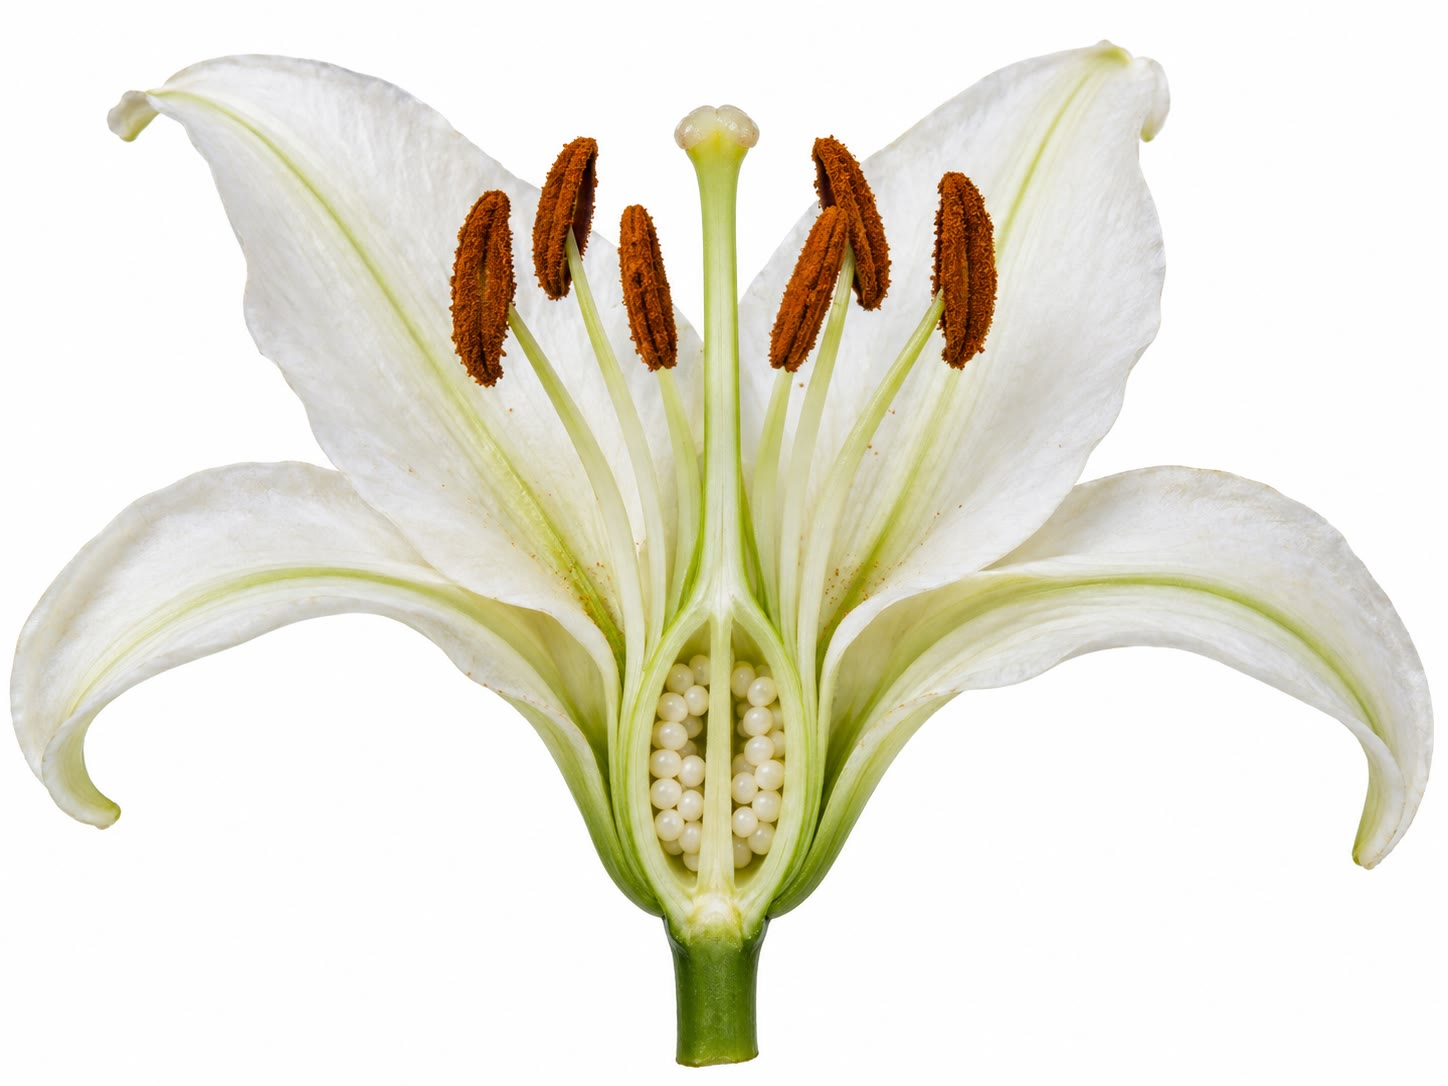
\includegraphics[width=0.55\linewidth]{images/book4/ai/b4-06-lily-dissected.jpg}

{\small زنبقة مشقوقة طولًا: ست سدى بمتوك محمّلة \omterm{def:b2:plant-life-cycles:heterospory}{باللقاح}، والقلم
الطويل بميسمه اللزج، والمبيض مفتوح ليُظهر صفوف البييضات.}
\end{omfigure}

\section{الطوران المشيجيان}

\begin{proposition}[حبة اللقاح: الطور المشيجي الذكري]\label{prop:b2:angiosperm-reproduction:pollen}
\index{حبة لقاح}\index{تكوّن الأبواغ الصغيرة}\index{سبوروبولينين}
في كل كيس \omterm{def:b2:plant-life-cycles:heterospory}{لقاح} تخضع خلايا أم ثنائية الصيغة \omterm{def:b2:meiosis-heredity:meiosis}{للتقسم المنصّف} فتعطي
رباعيات من \emph{الأبواغ الصغيرة}. وينقسم كل \omterm{def:b2:plant-life-cycles:heterospory}{بوغ صغير} مرة واحدة،
انقسامًا غير متساوٍ، إلى \emph{خلية خضرية} كبيرة و\emph{خلية مولّدة}
صغيرة محاطة بها؛ وتنقسم الخلية المولّدة مرة أخرى، قبل \omterm{def:b2:angiosperm-reproduction:pollination}{الإلقاح
اللقاحي} أو بعده، إلى \emph{خليتي نطفة}. فحبة \emph{\omterm{def:b2:plant-life-cycles:heterospory}{اللقاح}} الناضجة
كائن \omterm{def:b2:meiosis-heredity:meiosis}{فردي الصيغة} من ثلاث خلايا --- أي \omterm{def:b2:plant-life-cycles:cycles}{الطور المشيجي} الذكري كله ---
قياسه \qtyrange{10}{100}{\micro m}، مختوم في جدار طبقته الخارجية من
\emph{السبوروبولينين}، وهو أشد بوليمر حيوي معروف مقاومة، منحوتة
بأشواك ومسام وأخاديد مميزة للنوع، ولهذا يعرّف \omterm{def:b2:plant-life-cycles:heterospory}{اللقاح} النباتات في
رسابات عمرها عشرات ملايين السنين. وتُطلق الحبة منزوعة الماء، وتنجو
ساعات (النجيليات) إلى أسابيع (بعض الأشجار) حتى تبلغ ميسمًا.
\end{proposition}

\begin{omfigure}
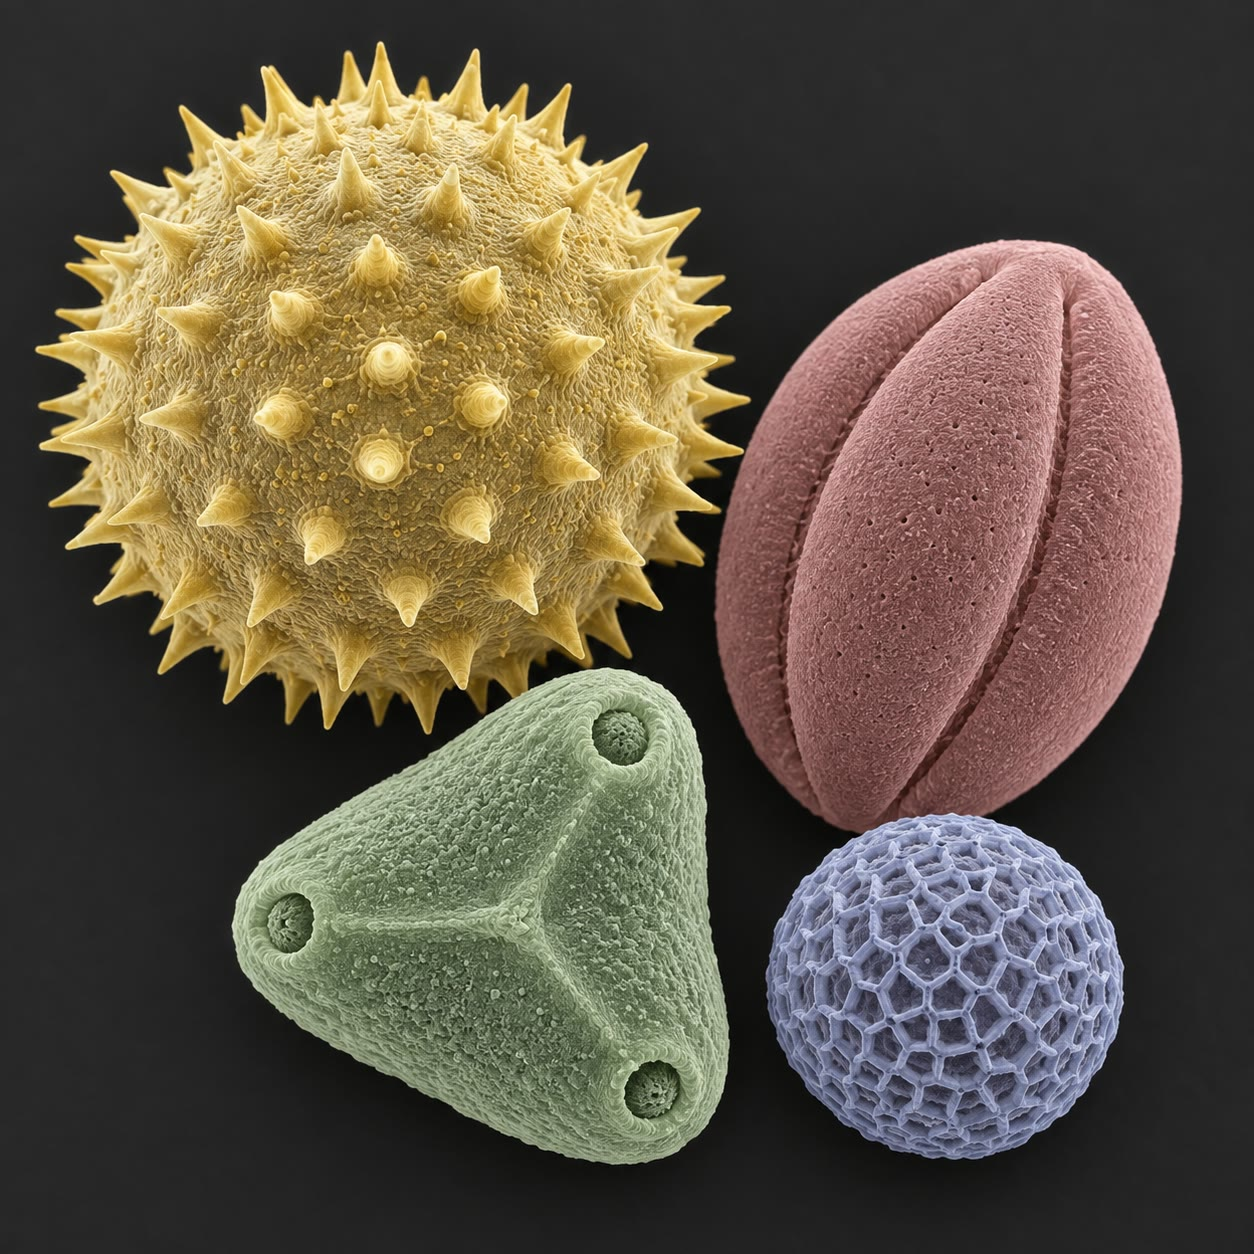
\includegraphics[width=0.45\linewidth]{images/book4/ai/b4-06-pollen-sem.jpg}

{\small حبوب \omterm{def:b2:plant-life-cycles:heterospory}{لقاح} تحت المجهر الإلكتروني الماسح: جدار
السبوروبولينين عند كل نوع له نحته الخاص --- أشواك، وأخاديد، ومسام،
وشبكة --- يُعرف به.}
\end{omfigure}

\begin{proposition}[الكيس الجنيني: الطور المشيجي الأنثوي]\label{prop:b2:angiosperm-reproduction:embryosac}
\index{كيس جنيني}\index{تكوّن الأبواغ الكبيرة}\index{نواتان قطبيتان}
في كل \omterm{def:b2:plant-life-cycles:heterospory}{بييضة} تخضع خلية ثنائية الصيغة من النوسيلة \omterm{def:b2:meiosis-heredity:meiosis}{للتقسم المنصّف}؛
فتنحل ثلاثة من الأبواغ الكبيرة الأربعة وينمو الرابع، بثلاثة تقسمات
خيطية بلا انقسام خلوي، إلى \emph{\omterm{prop:b2:angiosperm-reproduction:embryosac}{كيس جنيني}} ذي ثماني نوى وسبع
خلايا: عند الطرف النقيري \emph{البويضة}
يحفّ بها \emph{مرافقتان}؛ وعند الطرف البعيد ثلاث خلايا
\emph{مضادة}؛ وفي الوسط \emph{خلية مركزية} كبيرة
تحوي \emph{نواتين قطبيتين}. وهذا الكيس، ملفوفًا في النوسيلة
وغلافين فيهما نقير، هو \omterm{def:b2:plant-life-cycles:cycles}{الطور المشيجي} الأنثوي كله --- سبع خلايا حيث
كان \omterm{def:b2:plant-life-cycles:moss}{للطحلب} نبات. \omterm{prop:b2:angiosperm-reproduction:embryosac}{والنواتان القطبيتان} مطابقتان وراثيًا للبويضة، وهي
حقيقة تهم السويداء.
\end{proposition}

\begin{omfigure}
\begin{tikzpicture}[every node/.style={font=\scriptsize}]
  % pollen grain
  \begin{scope}
    \draw[very thick, omProp!80!black, fill=omProp!15] (0,0) circle (1.1);
    \draw[thick, omProp!80!black] (0,0) circle (0.95);
    \foreach \a in {0,30,...,330} \draw[omProp!80!black, thick] (\a:1.1) -- (\a:1.25);
    \draw[thick, fill=omDef!25] (0.15,-0.2) ellipse (0.55 and 0.4); \node[font=\tiny] at (0.15,-0.2) {خضرية};
    \draw[thick, fill=omThm!30] (-0.3,0.45) ellipse (0.22 and 0.14); \draw[thick, fill=omThm!30] (0.2,0.5) ellipse (0.22 and 0.14);
    \draw[omThm] (0.0,0.62) -- (0.0,1.5); \node[omThm, anchor=south] at (0.0,1.5) {خليتا نطفة};
    \node[below, align=center] at (0,-1.4) {حبة لقاح ($n$)\\3 خلايا، وجدار من السبوروبولينين};
  \end{scope}
  % ovule with embryo sac
  \begin{scope}[xshift=5.5cm]
    \draw[thick, fill=omExo!25] (0,0) ellipse (1.5 and 2.1);
    \draw[thick, fill=omExo!10] (0,0) ellipse (1.15 and 1.75);
    \fill[white] (-0.3,1.7) rectangle (0.3,2.2); \draw[thick] (-0.3,1.7) -- (-0.3,2.15); \draw[thick] (0.3,1.7) -- (0.3,2.15);
    \draw[thick, fill=white] (0,0) ellipse (0.7 and 1.35);
    % cells: egg + synergids top, central, antipodals bottom
    \draw[thick, fill=omThm!30] (0,0.95) circle (0.17); \node[omThm, anchor=west] at (1.6,1.2) {بويضة};
    \draw[thick, fill=omDef!25] (-0.35,1.0) circle (0.14); \draw[thick, fill=omDef!25] (0.35,1.0) circle (0.14); \node[anchor=west] at (1.6,0.75) {مرافقتان};
    \draw[thick, fill=omDef!10] (0,0) ellipse (0.55 and 0.6); \fill[omDef!80!black] (-0.15,0.05) circle (0.09); \fill[omDef!80!black] (0.15,0.05) circle (0.09);
    \node[anchor=west, align=left] at (1.6,0.1) {خلية مركزية بنواتين\\قطبيتين};
    \foreach \x in {-0.3,0,0.3} \draw[thick, fill=omDef!25] (\x,-1.0) circle (0.13); \node[anchor=west] at (1.6,-1.0) {ثلاث خلايا مضادة};
    \draw (0.35,2.0) -- (1.6,2.0) node[right] {نقير};
    \draw (1.3,-0.9) -- (1.6,-1.6) node[right] {غلافان};
    \draw (0.9,-1.35) -- (1.6,-2.1) node[right] {نوسيلة};
    \draw (1.6,1.2) -- (0.17,0.95); \draw (1.6,0.75) -- (0.49,1.0); \draw (1.6,0.1) -- (0.55,0.05); \draw (1.6,-1.0) -- (0.43,-1.0);
    \node[below, align=center] at (0,-2.3) {بييضة فيها كيس جنيني ($n$)\\7 خلايا، و8 نوى};
  \end{scope}
\end{tikzpicture}

{\small الطوران المشيجيان عند نبات زهري، وكلاهما منكمش إلى بضع
خلايا: \omterm{prop:b2:angiosperm-reproduction:pollen}{حبة اللقاح} الثلاثية الخلايا، \omterm{prop:b2:angiosperm-reproduction:embryosac}{والكيس الجنيني} السباعي الخلايا
داخل \omterm{def:b2:plant-life-cycles:heterospory}{البييضة}.}
\end{omfigure}

\section{الإلقاح اللقاحي}

\begin{definition}[الإلقاح اللقاحي وعوامله]\label{def:b2:angiosperm-reproduction:pollination}
\index{إلقاح لقاحي}\index{متلازمة الإلقاح اللقاحي}\index{رحيق}
\emph{الإلقاح اللقاحي} نقل \omterm{def:b2:plant-life-cycles:heterospory}{اللقاح} من متك إلى \omterm{def:b2:angiosperm-reproduction:flower}{ميسم}؛ فهو
\emph{ذاتي} داخل \omterm{def:b2:angiosperm-reproduction:flower}{زهرة} واحدة أو نبات واحد،
و\emph{خلطي} بين نباتين. والأزهار \emph{الملقحة بالرياح}
(النجيليات، والبلوط، والبتولا، ولسان الحمل) صغيرة خضراء
عديمة الرائحة، بمياسم كبيرة ريشية وكميات هائلة من \omterm{def:b2:plant-life-cycles:heterospory}{اللقاح} الأملس
الجاف؛ وتبلغ نسبة \omterm{def:b2:plant-life-cycles:heterospory}{اللقاح} إلى البييضات عندها المليون. أما الأزهار
\emph{الملقحة بالحيوانات} فتدفع لحاملها: \emph{رحيقًا}
(محلول سكر من غدد رحيقية)، أو لقاحًا نفسه، أو زيوتًا، أو عطرًا؛ وهي
تعلن بلون وشكل ورائحة مضبوطة على حواس الحامل --- أدلة رحيق فوق
بنفسجية للنحل الذي يرى فوق البنفسجي ولا يرى الأحمر؛ وأزهار أنبوبية
حمراء بلا رائحة للطنانات؛ وأزهار بيضاء عطرة بشدة تتفتح ليلًا
بأنابيب عميقة للعثّ؛ وأزهار بنية نتنة لذباب الجيف؛ وأزهار ليلية
شاحبة متينة للخفافيش. وكل طائفة من هذه الصفات \emph{متلازمة إلقاح
لقاحي}، والتوافق بين \omterm{def:b2:angiosperm-reproduction:flower}{الزهرة} والملقِّح هو المثال المدرسي على
\emph{التطور المشترك}: فقد تنبأ داروين من مهماز رحيق سحلبية مدغشقرية
طوله \qty{30}{cm} بعثّة لسانها \qty{30}{cm}، ووُجدت بعد أربعين سنة.
\end{definition}

\begin{omfigure}
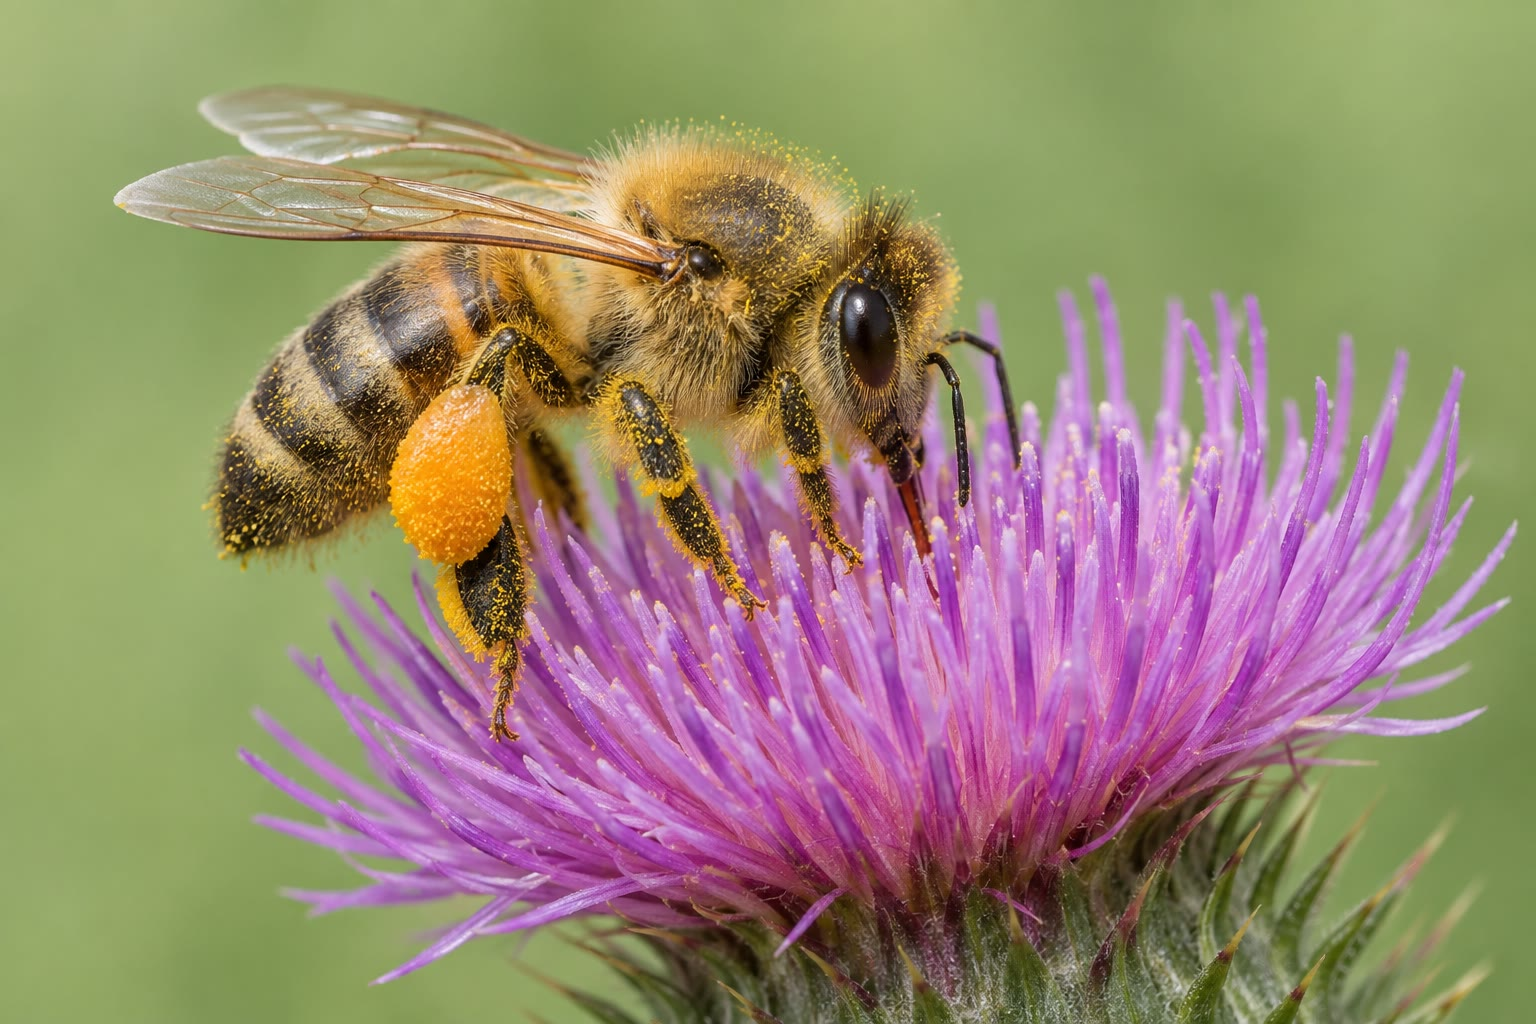
\includegraphics[width=0.58\linewidth]{images/book4/ai/b4-06-bee-on-flower.jpg}

{\small نحلة عسل على شوكة: يغبّر \omterm{def:b2:plant-life-cycles:heterospory}{اللقاح} جسمها ويحشو سلال ساقيها
الخلفيتين؛ وسيبلغ بعضه \omterm{def:b2:angiosperm-reproduction:flower}{ميسم} الشوكة التالية التي تزورها. فاللون
الأرجواني ومنصة الهبوط \omterm{def:b2:angiosperm-reproduction:pollination}{والرحيق} الغزير هي متلازمة النحل.}
\end{omfigure}

\begin{proposition}[تجنب الإلقاح الذاتي]\label{prop:b2:angiosperm-reproduction:selfing}
\index{عدم توافق ذاتي}\index{تغاير الأقلام}\index{تغاير النضج}
\omterm{def:b2:angiosperm-reproduction:flower}{الزهرة} الخنثى تستطيع أن تلقّح نفسها، وكثير منها يفعل (البازلاء،
والقمح، والبندورة)؛ لكن الإلقاح الذاتي يكشف الأليلات المتنحية
الضارة (\emph{ضعف التزاوج الداخلي})، ومعظم الأنواع تمنعه. ففي الزمن:
\emph{\omterm{prop:b2:angiosperm-reproduction:selfing}{تغاير النضج}}، إذ ينضج المتك \omterm{def:b2:angiosperm-reproduction:flower}{والميسم} في وقتين مختلفين (سبق
الذكورة عند معظم الخيميات والمركّبات). وفي الفراغ:
\emph{تباعد الأعضاء}، إذ يُبعد المتك عن \omterm{def:b2:angiosperm-reproduction:flower}{الميسم}، كما في
\emph{\omterm{prop:b2:angiosperm-reproduction:selfing}{تغاير الأقلام}} عند \omterm{def:b2:angiosperm-reproduction:flower}{زهرة} الربيع، حيث تضع أزهارها الطويلة القلم
(بمتوك منخفضة) وأزهارها القصيرة القلم (بمتوك مرتفعة) اللقاحَ
على مواضع مختلفة من الحشرة. وكيميائيًا حيويًا:
\emph{\omterm{prop:b2:angiosperm-reproduction:selfing}{عدم التوافق الذاتي}}، وهو جملة تعرّف يُرفض فيها \omterm{def:b2:plant-life-cycles:heterospory}{اللقاح} الحامل
\omterm{def:b2:meiosis-heredity:vocabulary}{أليل} $S$ مشتركًا مع المدقة. وفي عدم التوافق \emph{المشيجي}
(التفاح، والكرز، والبتونيا، والنجيليات) يقرر \omterm{def:b2:meiosis-heredity:vocabulary}{أليل} $S$ \omterm{def:b2:meiosis-heredity:meiosis}{الفردي الصيغة}
الخاص \omterm{def:b2:plant-life-cycles:heterospory}{باللقاح}: فمدقة $S_1S_2$ توقف أنابيب $S_1$ و$S_2$ في القلم،
فيكون \omterm{def:b2:plant-life-cycles:heterospory}{لقاح} نبات $S_1S_3$ متوافقًا بنصفه \omterm{def:b2:plant-life-cycles:heterospory}{ولقاح} $S_3S_4$ متوافقًا كله.
وفي عدم التوافق \emph{البوغي} (الملفوف، وعباد الشمس) يقرر \omterm{def:b2:meiosis-heredity:vocabulary}{النمط
الوراثي} \omterm{def:b2:meiosis-heredity:meiosis}{الثنائي الصيغة} لأبي \omterm{def:b2:plant-life-cycles:heterospory}{اللقاح}، على سطح \omterm{def:b2:angiosperm-reproduction:flower}{الميسم}. \omterm{def:b2:meiosis-heredity:vocabulary}{وأليل} $S$
النادر متوافق مع كل شريك تقريبًا، فيبقي الانتخاب عشرات الأليلات في
الجمهرة.
\end{proposition}
\begin{proof}[شواهد]
هجّن داروين (1862 و1877) زهور الربيع بيده: \omterm{def:b2:plant-life-cycles:heterospory}{فلقاح} \omterm{def:b2:angiosperm-reproduction:flower}{زهرة} قصيرة القلم
على \omterm{def:b2:angiosperm-reproduction:flower}{ميسم} \omterm{def:b2:angiosperm-reproduction:flower}{زهرة} طويلة القلم (وهو اتحاد «شرعي») عقد محافظ ممتلئة؛ أما
الطويلة على الطويلة أو القصيرة على القصيرة («غير الشرعي») فعقد بذورًا
قليلة أو لم يعقد، مع أن النباتات كانت سليمة \omterm{def:b2:plant-life-cycles:heterospory}{واللقاح} حيًا. فاستنتج
أن الشكلين متكيفان أحدهما مع الآخر للتهجين ومحميان من الإلقاح
الذاتي، وبعدّ البذور في المحفظة في آلاف التهجينات قاس كلفة الإلقاح
الذاتي في عشرات الأنواع: فالخلف الملقح ذاتيًا كان أقصر وأخف وأقل
خصوبة، جيلًا بعد جيل.
\end{proof}

\begin{omfigure}
\begin{tikzpicture}[every node/.style={font=\scriptsize}]
  % pistil S1S2 with pollen tubes
  \draw[thick, fill=omDef!10] (-0.5,0) rectangle (0.5,3.2);
  \draw[thick, fill=omDef!30] (0,3.3) ellipse (0.7 and 0.2);
  \draw[thick, fill=omDef!12] (0,-0.6) ellipse (0.9 and 0.7);
  \node at (0,-0.6) {مبيض};
  \node[anchor=east] at (-1.1,3.3) {ميسم نبات $S_1S_2$};
  % pollen grains
  \draw[thick, fill=omThm!40] (-0.35,3.75) circle (0.13); \node[omThm, left] at (-0.5,3.75) {$S_1$};
  \draw[thick, fill=omThm!40] (0,3.75) circle (0.13); \node[omThm, anchor=south] at (0,3.92) {$S_2$};
  \draw[thick, fill=omExo!70!black] (0.35,3.75) circle (0.13); \node[right] at (0.5,3.75) {$S_3$};
  % tubes: S1 and S2 stop in the style, S3 reaches the ovary
  \draw[thick, omThm] (-0.35,3.3) -- (-0.35,2.3); \node[omThm, left, align=right] at (-0.55,2.3) {أنبوب $S_1$\\موقوف};
  \draw[thick, omThm] (0,3.3) -- (0,2.0);
  \draw[thick, omExo!70!black] (0.35,3.3) -- (0.35,-0.2) -- (0.2,-0.5);
  \node[right, align=left] at (0.55,0.9) {أنبوب $S_3$\\يبلغ بييضة};
  \node[anchor=west, align=left, text width=6cm] at (3.2,3.2) {عدم توافق ذاتي مشيجي: أنبوب اللقاح الذي يطابق أليله $S$ أحد أليلي المدقة يُوقف في القلم};
  \node[anchor=west, align=left, text width=6cm] at (3.2,1.4) {لقاح نبات $S_1S_2$: لا متوافق\\ومن $S_1S_3$: النصف\\ومن $S_3S_4$: الكل};
\end{tikzpicture}

{\small \omterm{prop:b2:angiosperm-reproduction:selfing}{عدم التوافق الذاتي} المشيجي. على مدقة $S_1S_2$، تُوقف
الأنابيب الحاملة $S_1$ أو $S_2$ في القلم؛ أما أنبوب $S_3$
فينمو إلى المبيض.}
\end{omfigure}

\section{الإلقاح}

\begin{theorem}[أنبوب اللقاح]\label{thm:b2:angiosperm-reproduction:tube}
\index{أنبوب لقاح}
\omterm{prop:b2:angiosperm-reproduction:pollen}{حبة اللقاح} على \omterm{def:b2:angiosperm-reproduction:flower}{ميسم} متوافق تستعيد ماءها وتنمي
\emph{\omterm{thm:b2:angiosperm-reproduction:tube}{أنبوب لقاح}}: فتمتد الخلية الخضرية بنمو قمي،
واضعةً جدارًا جديدًا عند القمة بمعدل \qtyrange{0.1}{1}{cm/h}،
هاضمةً طريقها عبر النسيج الناقل في القلم ومتغذيةً عليه. ويحمل
الأنبوب خليتي النطفة عند قمته؛ وتهديه في المسافة الأخيرة ببتيدات
تفرزها المرافقتان، فيدخل \omterm{def:b2:plant-life-cycles:heterospory}{البييضة} عبر النقير، وينفجر في إحدى
المرافقتين، ويطلق النطفتين. والأنبوب الذي يعبر قلمًا طوله $L$
بسرعة $v$ يستغرق $L/v$: أي بضع ساعات عند الكرز، ويومًا كاملًا عند
الذرة التي «حريرها» أقلام طولها \qty{20}{cm}. وحيوية \omterm{def:b2:plant-life-cycles:heterospory}{اللقاح} تضبط
ساعةً: \omterm{def:b2:plant-life-cycles:heterospory}{فلقاح} النجيليات يموت في ساعات، فلا بد من بلوغ \omterm{def:b2:angiosperm-reproduction:flower}{ميسم} بسرعة.
\end{theorem}
\begin{proof}
الزمن هو الطول مقسومًا على معدل النمو؛ فعند الذرة، تعطي
\qty{20}{cm} عند \qty{1}{cm/h} مقدار \qty{20}{h}. والأنبوب نفسه
يتألف كله تقريبًا من جدار وغشاء رقيق من السيتوبلازم خلف القمة،
فتكفي مؤونة الخلية الخضرية، مع ما تمتصه من القلم، لطول يعادل ألف
مرة قطر الحبة.
\end{proof}

\begin{proposition}[الإلقاح المضاعف]\label{prop:b2:angiosperm-reproduction:double}
\index{إلقاح مضاعف}\index{سويداء}
من خليتي النطفة اللتين يسلّمهما الأنبوب، تندمج إحداهما بالبويضة
فتكوّن \emph{اللاقحة} الثنائية الصيغة التي ينمو منها الجنين؛
وتندمج الأخرى بالخلية المركزية ونواتيها القطبيتين فتكوّن نواة
\emph{ثلاثية الصيغة} ($3n$: مورثومان أموميان وواحد أبوي)، ينمو منها
\emph{السويداء} --- وهو نسيج مغذٍّ يملأ \omterm{def:b2:angiosperm-reproduction:seed}{البذرة} بالنشاء والزيت
والبروتين. ويقع الإلقاحان خلال دقائق أحدهما من الآخر؛ ولا ينجح
أحدهما دون الآخر في معظم الأنواع، فلا يموّن النبات إلا البذور التي
تحمل جنينًا. والسويداء هو النسيج الذي يطعم البشرية: فطحين القمح
والأرز، ودقيق الذرة، وأبيض جوز الهند سويداء ثلاثي الصيغة. أما عند
عاريات البذور فمخزون غذاء \omterm{def:b2:angiosperm-reproduction:seed}{البذرة} هو \omterm{def:b2:plant-life-cycles:cycles}{الطور المشيجي} الأنثوي، المبني
قبل الإلقاح سواء تلاه جنين أم لا؛ وسويداء كاسيات البذور يُصنع
حسب الطلب.
\end{proposition}
\begin{proof}[شواهد]
تتبع ناواشين (1898) \omterm{thm:b2:angiosperm-reproduction:tube}{أنبوب لقاح} زنبقة وفريتيلاريا إلى \omterm{prop:b2:angiosperm-reproduction:embryosac}{الكيس الجنيني}
تحت المجهر، فرأى نواتي النطفتين تغادران الأنبوب، إحداهما تدخل
البويضة والأخرى تندمج بالنواتين القطبيتين؛ وأكد ذلك غينيار في السنة
التالية عند أنواع أخرى. وتبعت ثلاثية صيغة السويداء من عدّ
الصبغيات، أما نتائجها الوراثية --- أي أن سويداء الحبة يُظهر صفات أبي
\omterm{def:b2:plant-life-cycles:heterospory}{اللقاح} (\emph{الغريبية})، بنسبة جرعتين
أموميتين إلى جرعة أبوية --- فكان مربّو الذرة قد لاحظوها قبل ذلك
بزمن طويل.
\end{proof}

\begin{omfigure}
\begin{tikzpicture}[every node/.style={font=\scriptsize}, >=stealth]
  \node[draw, rounded corners, fill=omProp!15, align=center] (sp) at (0,2) {خلية نطفة 1 ($n$)};
  \node[draw, rounded corners, fill=omProp!15, align=center] (sp2) at (0,0) {خلية نطفة 2 ($n$)};
  \node[draw, rounded corners, fill=omThm!15, align=center] (egg) at (4,2) {بويضة ($n$)};
  \node[draw, rounded corners, fill=omDef!15, align=center] (cc) at (4,0) {خلية مركزية\\نواتان قطبيتان ($n + n$)};
  \node[draw, rounded corners, fill=omThm!30, align=center] (zyg) at (8.6,2) {لاقحة ($2n$)\\$\to$ جنين};
  \node[draw, rounded corners, fill=omDef!30, align=center] (endo) at (8.6,0) {نواة السويداء ($3n$)\\$\to$ سويداء، وهو مخزون الغذاء};
  \draw[->, thick] (sp) -- (egg); \draw[->, thick] (egg) -- (zyg);
  \draw[->, thick] (sp2) -- (cc); \draw[->, thick] (cc) -- (endo);
  \node[anchor=south] at (2,2.5) {الإلقاح 1};
  \node[anchor=south] at (2,0.5) {الإلقاح 2};
  \node[anchor=north, align=center] at (4.3,-0.9) {أنبوب لقاح واحد، وخليتا نطفة، واندماجان: فيُصنع الجنين ومؤونته معًا};
\end{tikzpicture}

{\small \omterm{prop:b2:angiosperm-reproduction:double}{الإلقاح المضاعف}: نطفة تصنع اللاقحة الثنائية الصيغة،
والأخرى تصنع السويداء الثلاثي الصيغة.}
\end{omfigure}

\section{البذرة والثمرة}

\begin{definition}[من البييضة إلى البذرة، ومن المبيض إلى الثمرة]\label{def:b2:angiosperm-reproduction:seed}
\index{بذرة}\index{ثمرة}\index{فلقة}\index{سكون}
تنقسم اللاقحة إلى معلاق يدفع الجنين إلى داخل السويداء، وجنين حقيقي
يمر بأطوار كروي وقلبي ومغزلي وهو يضع قطبي الجذر والساق و\emph{فلقة}
أو فلقتين (أوراق بذرية) --- وهو تمييز أحادي الفلقة من ثنائيها. وفي
كثير من ثنائيات الفلقة (الفاصولياء والبازلاء) تمتص الفلقات النامية
السويداء وتصير هي مخزون الغذاء؛ أما في الحبوب ومعظم أحاديات الفلقة
فيبقى السويداء وتكون الفلقة الوحيدة عضو امتصاص. ويتصلب الغلافان
فيصيران \emph{قشرة البذرة}؛ وتفقد البذرة ماءها حتى \qtyrange{5}{15}{\%}،
ويتوقف الاستقلاب، وتدخل في \emph{سكون} لا ينتهي إلا حين تقول
إشارة --- ماء، أو برد، أو ضوء، أو نار، أو مرور في أمعاء --- إن
الموسم مواتٍ. وفي تلك الأثناء ينمو جدار المبيض
\emph{ثمرةً} شكلها استراتيجية انتشار: ثمار جافة تنشق
(القرون والمحافظ) أو لا تنشق (الحبوب والجوزات والسمرات
المجنحة)، وثمار لحمية تُؤكل (العنبات، والحسلات ذات النواة،
والتفاحة التي لحمها تخت)؛ وتمر البذرة في الحيوان سالمة، وقد خُدشت
قشرتها، وتُودع مع سماد على بعد كيلومترات.
\end{definition}
\begin{proof}[شواهد]
تبين حبة الحبوب كيف يُضبط الإنبات. فالجنين، حين يشرب الماء، يفرز
الجبريلين في السويداء المحيط به؛ فتستجيب الطبقة الخارجية من
السويداء، وهي الألورون، بصنع $\alpha$-أميلاز وإفرازه، وهو يهضم
النشاء إلى سكريات يمتصها الجنين. أما أنصاف الحبات التي بلا جنين فلا
تصنع أميلازًا؛ فإذا أُضيف إليها الجبريلين صنعته (باليغ ويومو، 1960)؛
والهرمون يعمل بإشعال مورّثة الأميلاز، وهي من أوائل الحالات التي
اقتُفي فيها هرمون نباتي إلى مورّثة. وقد استعمل صانعو الجعة العملية
منذ آلاف السنين: فالتمليت شعير أُنبت ثم جُفّف.
\end{proof}

\begin{omfigure}
\begin{tikzpicture}[every node/.style={font=\scriptsize}]
  % embryogenesis stages
  \foreach \x/\lab in {0/{لاقحة}, 1.6/{خليتان}, 3.4/{كروي}, 5.6/{قلبي}, 8.2/{مغزلي}} \node[below] at (\x,-1.1) {\lab};
  \draw[thick, fill=omThm!25] (0,-0.2) circle (0.22);
  \draw[thick, fill=omThm!25] (1.6,0.0) circle (0.2); \draw[thick, fill=omDef!15] (1.6,-0.45) circle (0.14);
  \draw[thick, fill=omThm!25] (3.4,0.1) circle (0.45); \foreach \y in {-0.5,-0.75,-1.0} \draw[thick, fill=omDef!15] (3.4,\y) circle (0.1);
  \draw[thick, fill=omThm!25] (5.6,0.0) .. controls (4.9,1.0) and (5.2,-0.6) .. (5.6,-0.6) .. controls (6.0,-0.6) and (6.3,1.0) .. (5.6,0.0);
  \draw[thick, fill=omThm!25] (5.15,0.5) circle (0.32); \draw[thick, fill=omThm!25] (6.05,0.5) circle (0.32);
  \foreach \y in {-0.75,-1.0} \draw[thick, fill=omDef!15] (5.6,\y) circle (0.09);
  \draw[thick, fill=omThm!25] (8.2,-0.2) ellipse (0.3 and 0.75);
  \draw[thick, fill=omThm!25] (7.75,0.9) .. controls (7.4,1.6) and (7.9,1.9) .. (8.05,0.55) -- cycle;
  \draw[thick, fill=omThm!25] (8.65,0.9) .. controls (9.0,1.6) and (8.5,1.9) .. (8.35,0.55) -- cycle;
  \node[omDef!80!black, anchor=west] at (9.3,-0.9) {معلاق (بالأزرق)};
  \node[omThm, anchor=west] at (9.3,0.9) {فلقتان};
  \node[anchor=west] at (9.3,-0.2) {قطب الجذر في الأسفل};
\end{tikzpicture}

{\small تكوّن الجنين عند ثنائي \omterm{def:b2:angiosperm-reproduction:seed}{الفلقة}: تنقسم اللاقحة إلى جنين
ومعلاق؛ ويصير الجنين الكروي قلبي الشكل حين تبرز الفلقتان، ثم
مغزليًا حين يمتد محور الجذر والساق.}
\end{omfigure}

\begin{omfigure}
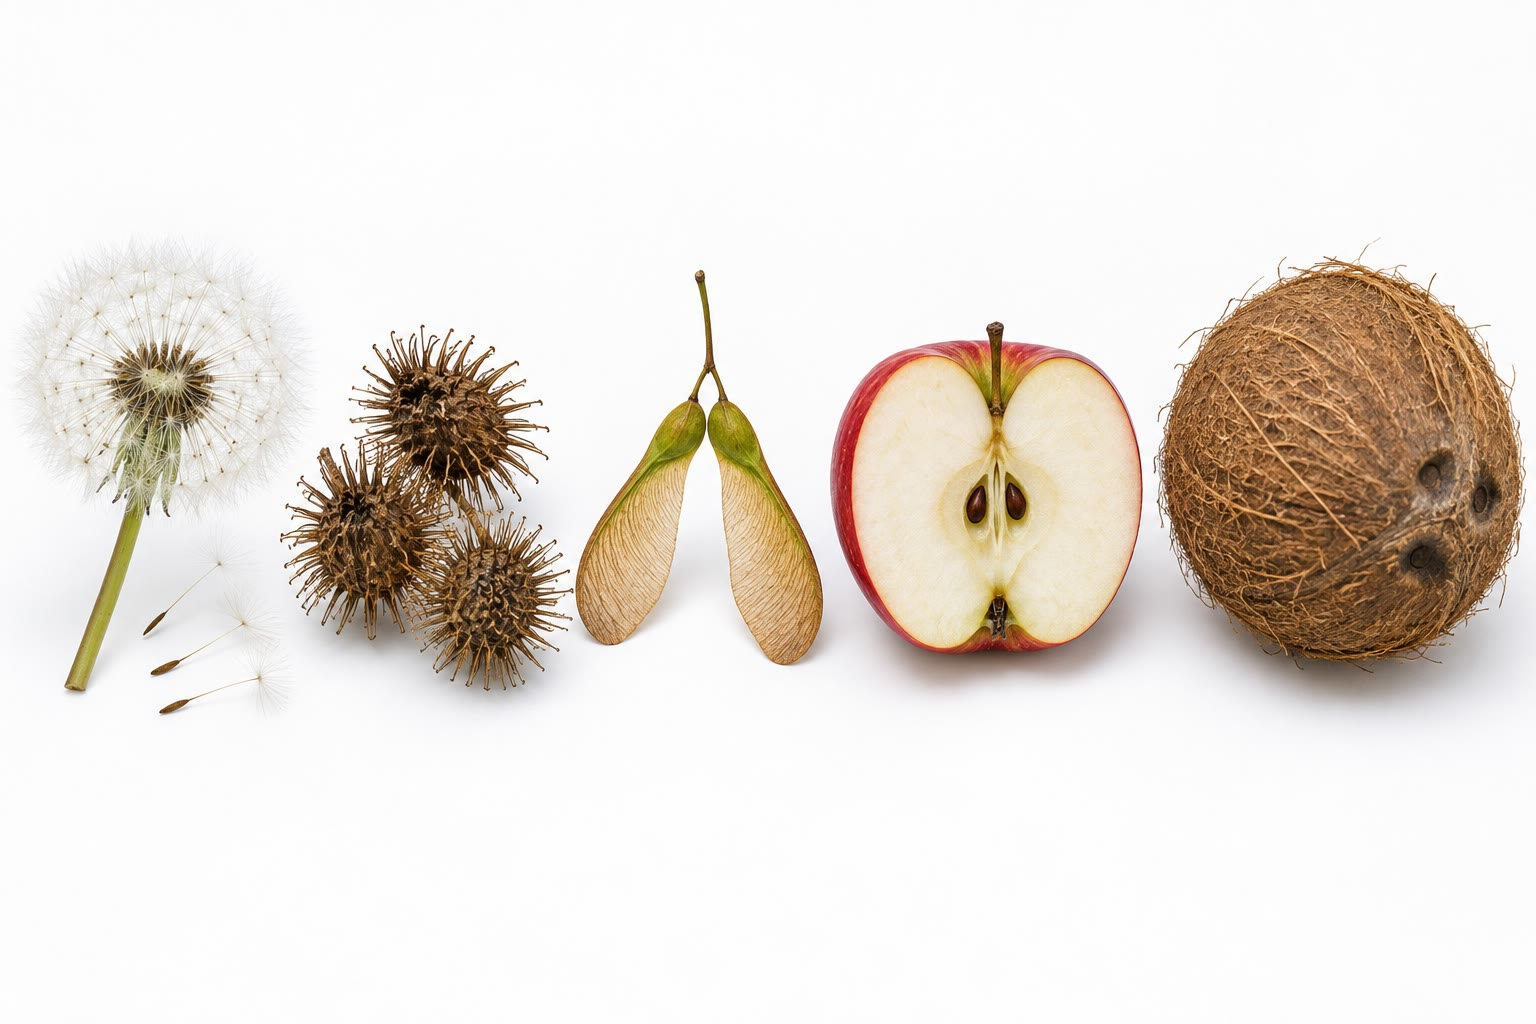
\includegraphics[width=0.62\linewidth]{images/book4/ai/b4-06-fruits-seeds.jpg}

{\small ثمار مبنية للانتشار: مظلات (الهندباء)، وخطاطيف (الأرقطيون)،
وأجنحة (القيقب)، ولحم لحيوان (التفاح)، وقشرة طافية للبحر (جوز
الهند).}
\end{omfigure}

\begin{example}[مسافات الانتشار]\label{ex:b2:angiosperm-reproduction:dispersal}
فُقيرة هندباء بمظلتها تهبط بسرعة \qty{0.3}{m/s}؛ ومن \qty{0.3}{m} في
رياح سرعتها \qty{3}{m/s} تطير \qty{3}{m}، وفي تيار حراري صاعد تطير
مئات الأمتار. وسمرة قيقب تهبط بدورانها الذاتي بسرعة
\qty{1}{m/s} من \qty{15}{m}: أي \qty{45}{m}. ونواة كرز يسقطها طائر
بعد طيران عشرين دقيقة بسرعة \qty{10}{m/s}: تبلغ
\qty{12}{km}. أما جوز البلوط فيسقط عند قدم الشجرة ما لم يحمله قيق،
وهو يفعل ذلك بالآلاف، إلى كيلومتر وأكثر، وينسى عُشره: فأشجار البلوط
التي أعادت استعمار أوروبا بعد العصر الجليدي الأخير تحركت شمالًا
مئات الأمتار في السنة، أسرع بكثير مما تتدحرج به جوزة، والطيور هي
التي حركتها.
\end{example}

\section{تمارين}

\begin{exercise}[$\star$]\label{exo:b2:angiosperm-reproduction:1}
سمِّ دوّارات \omterm{def:b2:angiosperm-reproduction:flower}{الزهرة} الأربع وأجزاء \omterm{def:b2:angiosperm-reproduction:flower}{السداة} \omterm{def:b2:angiosperm-reproduction:flower}{والكربلة}. وأي الأجزاء \omterm{def:b2:plant-life-cycles:cycles}{طور
بوغي} \omterm{def:b2:meiosis-heredity:meiosis}{ثنائي الصيغة}، وأيها \omterm{def:b2:plant-life-cycles:cycles}{طور مشيجي} \omterm{def:b2:meiosis-heredity:meiosis}{فردي الصيغة}؟
\end{exercise}

\begin{exercise}[$\star$]\label{exo:b2:angiosperm-reproduction:2}
أعط صيغة الصبغيات لكل من: \omterm{def:b2:plant-life-cycles:heterospory}{بوغ صغير}، والخلية الخضرية، وخلية نطفة،
والبويضة، ونواة قطبية، واللاقحة، والسويداء، \omterm{def:b2:angiosperm-reproduction:seed}{وقشرة البذرة}، وجدار
\omterm{def:b2:angiosperm-reproduction:seed}{الثمرة}.
\end{exercise}

\begin{exercise}[$\star$]\label{exo:b2:angiosperm-reproduction:3}
اذكر خمس صفات \omterm{def:b2:angiosperm-reproduction:flower}{لزهرة} ملقحة بالرياح وخمسًا \omterm{def:b2:angiosperm-reproduction:flower}{لزهرة} ملقحة بالنحل، وأعط
نباتًا لكل منهما.
\end{exercise}

\begin{exercise}[$\star$]\label{exo:b2:angiosperm-reproduction:4}
ما \omterm{prop:b2:angiosperm-reproduction:double}{الإلقاح المضاعف}، وما الذي يصنعه كل من الاندماجين؟ ولماذا يمكن
وصف السويداء بأنه «مصنوع حسب الطلب»؟
\end{exercise}

\begin{exercise}[$\star\star$]\label{exo:b2:angiosperm-reproduction:5}
حريرة ذرة طولها \qty{25}{cm} \omterm{thm:b2:angiosperm-reproduction:tube}{وأنبوب اللقاح} ينمو بسرعة
\qty{1.2}{cm/h}. فكم يستغرق الإلقاح بعد \omterm{def:b2:angiosperm-reproduction:pollination}{الإلقاح اللقاحي}؟
وتنثر النورة الذكرية \omterm{def:b2:plant-life-cycles:heterospory}{اللقاح} من اليوم 0 إلى اليوم 7 وتبرز حرائر
النبات من اليوم 5 إلى اليوم 12، ثُمنها في كل يوم؛ ولا تلتقط
الحريرة لقاحًا إلا ما دام \omterm{def:b2:plant-life-cycles:heterospory}{اللقاح} يُنثر. فما كسر الحرائر الملقحة؟
\end{exercise}

\begin{exercise}[$\star\star$]\label{exo:b2:angiosperm-reproduction:6}
في \omterm{prop:b2:angiosperm-reproduction:selfing}{عدم التوافق الذاتي} المشيجي، ما كسر \omterm{def:b2:plant-life-cycles:heterospory}{اللقاح} المتوافق في التهجينات
$S_1S_2\times S_1S_2$ و$S_1S_2\times
S_1S_3$ و$S_1S_2\times S_3S_4$ (والمدقة مذكورة أولًا)؟ أعط
الأنماط الوراثية لخلف التهجين الثاني.
\end{exercise}

\begin{exercise}[$\star\star$]\label{exo:b2:angiosperm-reproduction:7}
في جمهرة فيها $n$ \omterm{def:b2:meiosis-heredity:vocabulary}{أليل} $S$ متساوية التواتر، ما كسر \omterm{def:b2:plant-life-cycles:heterospory}{اللقاح} العشوائي
المتوافق مع نبات معين؟ واشرح لماذا ينتشر \omterm{def:b2:meiosis-heredity:vocabulary}{أليل} $S$ جديد ينشأ
\omterm{def:b2:genome-diversification:mutation}{بالطفرة}، وبماذا يتنبأ هذا في عدد الأليلات.
\end{exercise}

\begin{exercise}[$\star\star$]\label{exo:b2:angiosperm-reproduction:8}
نبات ذرة \omterm{def:b2:meiosis-heredity:vocabulary}{متغاير اللواقح} $Yy$ (وسويداؤه الأصفر \omterm{def:b2:meiosis-heredity:vocabulary}{سائد}) لُقّح ذاتيًا.
أعط الأنماط الوراثية لسويداء حباته ونسبها، متذكرًا أن النواتين
القطبيتين متطابقتان. فما كسر الحبات الصفراء؟ وماذا لو لُقّح النبات
\omterm{def:b2:plant-life-cycles:heterospory}{بلقاح} نبات $yy$؟
\end{exercise}

\begin{exercise}[$\star\star$]\label{exo:b2:angiosperm-reproduction:9}
صف تجربة الألورون واشرح ما تبينه عن (أ) دور الجنين، (ب) ودور
الجبريلين، (ج) وموضع اصطناع الأميلاز. ولماذا يكون نصف الحبة بلا
جنين هو الشاهد الجوهري؟
\end{exercise}

\begin{exercise}[$\star\star\star$]\label{exo:b2:angiosperm-reproduction:10}
قارن استراتيجيتي الرياح والحيوان من جهة الكلفة: فنبات ملقح بالرياح
يصنع $10^{6}$ حبة لكل \omterm{def:b2:plant-life-cycles:heterospory}{بييضة} كتلة كل منها \qty{1}{\micro g}؛ ونبات
ملقح بالحيوانات يصنع $10^{3}$ حبة لكل \omterm{def:b2:plant-life-cycles:heterospory}{بييضة} كتلة كل منها
\qty{1}{\micro g} زائد \qty{5}{mg} من سكر \omterm{def:b2:angiosperm-reproduction:pollination}{الرحيق} لكل \omterm{def:b2:angiosperm-reproduction:flower}{زهرة}
فيها عشر بييضات. احسب كلفة التكاثر لكل \omterm{def:b2:plant-life-cycles:heterospory}{بييضة} في الحالتين
(خذ \omterm{def:b2:plant-life-cycles:heterospory}{اللقاح} والسكر بالطاقة نفسها لكل غرام)، واشرح لماذا يبقى
الإلقاح بالرياح مع ذلك.
\end{exercise}

\begin{exercise}[$\star\star\star$]\label{exo:b2:angiosperm-reproduction:11}
اشرح، بأرقام \cref{ex:b2:angiosperm-reproduction:dispersal}،
لماذا تستحق \omterm{def:b2:angiosperm-reproduction:seed}{الثمرة} اللحمية كلفتها عند الشجرة مع أن
الحيوان يهضم اللحم ويسقط معظم البذور حيث لا تستطيع النمو.
\end{exercise}

\begin{exercise}[$\star\star\star$]\label{exo:b2:angiosperm-reproduction:12}
«\omterm{def:b2:angiosperm-reproduction:flower}{الكربلة} المغلقة هي سبب سيادة النباتات الزهرية على اليابسة.» ناقش
هذا: ما الذي تتيحه إحاطة \omterm{def:b2:plant-life-cycles:heterospory}{البييضة} (اختيار \omterm{def:b2:plant-life-cycles:heterospory}{اللقاح}، وعدم التوافق،
\omterm{def:b2:angiosperm-reproduction:seed}{والثمرة}) وما الذي تكلفه.
\end{exercise}

\section{مسألة: بستان وحقل}

\begin{problem}[{مسألة نهاية الأسبوع --- تخطيط الإلقاح اللقاحي في
بستان تفاح حول عدم التوافق الذاتي، وحساب إلقاح حقل ذرة ومردوده من
اللقاح الذي يصنعه، وتنتهي إلى عقد ثمار البستان وعدد حبات الحقل}]
\label{pb:b2:angiosperm-reproduction:1}
التفاح غير متوافق ذاتيًا توافقًا مشيجيًا. وفي بستان ثلاثة
أصناف: A ($S_1S_2$)، وB ($S_1S_3$)، وC ($S_3S_4$). وللزهرة خمس
كرابل في كل منها بييضتان، \omterm{def:b2:angiosperm-reproduction:seed}{والثمرة} التي تعقد أقل من خمس بذور تسقطها
الشجرة. وزيارة نحلة تودع \num{100} \omterm{prop:b2:angiosperm-reproduction:pollen}{حبة لقاح}
على \omterm{def:b2:angiosperm-reproduction:flower}{ميسم}؛ ولكل حبة متوافقة احتمال $0.1$ في
إلقاح \omterm{def:b2:plant-life-cycles:heterospory}{بييضة} لم تُؤخذ بعد. وتحمل الشجرة \num{5000} \omterm{def:b2:angiosperm-reproduction:flower}{زهرة}
وتحتاج إلى \num{250} \omterm{def:b2:angiosperm-reproduction:seed}{ثمرة} لمحصول كامل. والذرة: تنثر النورة الذكرية
$10^{7}$ حبة على مدى \num{7} أيام؛ ويضم الحقل \num{8} نباتات في
المتر المربع؛ ويحمل النبات كوزًا واحدًا فيه \num{600} حريرة؛
وتقدّم الحريرة \qty{1e-4}{m^2} \omterm{def:b2:plant-life-cycles:heterospory}{للقاح} الهابط؛ ويترسب \omterm{def:b2:plant-life-cycles:heterospory}{اللقاح} بسرعة
\qty{0.25}{m/s}؛ وتحوي الحبة \qty{0.3}{g} من السويداء.

\medskip
\noindent\textbf{الجزء الأول --- التوافق.}
\begin{enumerate}
  \item من أجل \omterm{def:b2:plant-life-cycles:heterospory}{لقاح} كل صنف على مدقة A، أعط الكسر المتوافق $f$.
  \item الشيء نفسه من أجل مدقتي B وC.
  \item نحلة قادمة من شجرة B تودع 100 حبة على \omterm{def:b2:angiosperm-reproduction:flower}{ميسم} A: فكم منها
        متوافق، وكم \omterm{def:b2:plant-life-cycles:heterospory}{بييضة} يُنتظر إلقاحها (أهمل الإشباع)؟
  \item الشيء نفسه من أجل نحلة من C، ومن شجرة A أخرى.
  \item أي الثمار تُبقى؟ وما خطر غرس بستان من الصنف A وحده؟
  \item كتلة من أشجار A تحيط بها أشجار C؛ ونصف زيارات النحل إلى A
        تأتي من C. فإذا تلقت كل \omterm{def:b2:angiosperm-reproduction:flower}{زهرة} زيارة واحدة، فما كسر أزهار A
        التي تعقد ثمرًا، وكم \omterm{def:b2:angiosperm-reproduction:seed}{ثمرة} في الشجرة؟ وهل المحصول كامل؟
  \item لماذا تُغرس في البساتين تفاحة برية تزهر أسابيع، ولماذا يجب
        فحص أليلات $S$ عندها؟
\end{enumerate}

\medskip
\noindent\textbf{الجزء الثاني --- \omterm{def:b2:plant-life-cycles:heterospory}{اللقاح} فوق حقل الذرة.}
\begin{enumerate}[resume]
  \item احسب \omterm{def:b2:plant-life-cycles:heterospory}{اللقاح} المطلوق من المتر المربع من الحقل في الثانية،
        وسطيًا على مدى الأيام السبعة.
  \item في الحالة المستقرة يساوي تدفق \omterm{def:b2:plant-life-cycles:heterospory}{اللقاح} المترسب معدل الإطلاق.
        احسب تركيز \omterm{def:b2:plant-life-cycles:heterospory}{اللقاح} في الهواء (حبات في المتر المكعب).
  \item احسب عدد الحبات التي تحط على حريرة واحدة في الثانية،
        ومتوسط زمن الانتظار لأول حبة.
  \item كم حبة تتلقى الحريرة في اليوم؟ ولماذا لا تفيد إلا الأولى؟
  \item حريرة طولها \qty{20}{cm} لُقّحت؛ والأنبوب ينمو بسرعة
        \qty{1}{cm/h}. فمتى تُلقّح \omterm{def:b2:plant-life-cycles:heterospory}{البييضة}؟
  \item يؤخر جفاف بروزَ الحرائر خمسة أيام بينما تنثر النورة
        الذكرية في موعدها. قدّر، بفترة النثر البالغة سبعة أيام،
        كسر موسم \omterm{def:b2:plant-life-cycles:heterospory}{اللقاح} الذي تلتقطه الحرائر، والعاقبة على المردود.
\end{enumerate}

\medskip
\noindent\textbf{الجزء الثالث --- \omterm{prop:b2:angiosperm-reproduction:double}{الإلقاح المضاعف} والحبة.}
الحقل من صنف سويداؤه أصفر ($Y$، \omterm{def:b2:meiosis-heredity:vocabulary}{سائد}) بجوار حقل أبيض ($yy$)؛
والرياح تهب من الحقل الأبيض.
\begin{enumerate}[resume]
  \item أعط النمطين الوراثيين لجنين حبة نبات $YY$ لُقّح \omterm{def:b2:plant-life-cycles:heterospory}{بلقاح} $yy$
        ولسويدائها.
  \item هل الحبة صفراء أم بيضاء؟ واشرح مصطلح الغريبية.
  \item نبات $Yy$ لُقّح \omterm{def:b2:plant-life-cycles:heterospory}{بلقاح} $yy$: أعط الأنماط الوراثية للسويداء
        وتواتراتها.
  \item يحوي السويداء مورثومين أموميين وواحدًا أبويًا.
        ومورّثة ذات أثر جرعي تعطي 10~وحدات صبغة لكل نسخة: فأي صبغة
        تحملها الحبات $YYy$ و$Yyy$ و$yyY$
        (بجرعتين أبويتين فرضًا)؟ وأي هذه يمكن أن يوجد فعلًا؟
  \item اشرح لماذا يكون السويداء، لا الجنين، هو ما نأكله، وما كسر
        كتلة الحبة الذي يمثله إذا كان الجنين يزن \qty{0.03}{g}.
  \item لماذا يكون تموين السويداء «حسب الطلب» ميزة على تموين عاريات
        البذور؟
\end{enumerate}

\medskip
\noindent\textbf{الجزء الرابع --- المردود.}
\begin{enumerate}[resume]
  \item إذا لُقّحت \qty{90}{\%} من الحرائر، احسب عدد الحبات في
        الكوز وفي النبات وفي المتر المربع، وكتلة السويداء في المتر
        المربع.
  \item حوّل ذلك إلى أطنان في الهكتار.
  \item يثبّت المحصول \qty{1.2}{kg} من الكربون في المتر المربع في
        الموسم، ينتهي نصفها في الحبوب المحصودة. تحقق من الاتساق مع
        كتلة السؤال 20 (والسويداء \qty{45}{\%} كربونًا).
  \item كم \omterm{prop:b2:angiosperm-reproduction:pollen}{حبة لقاح} نثر الحقل لكل حبة محصودة؟
  \item اشرح لماذا يعقد نبات ذرة منفرد في حديقة كوزًا سيئ الامتلاء.
  \item اذكر النتيجة: عقد ثمار كتلة A، ومردود الحقل بالحبات في
        المتر المربع وبالأطنان في الهكتار.
\end{enumerate}
\end{problem}
